\renewcommand{\graphscale}{0.8}

\begin{algorithm}[htb]
   \caption{C4}
   \label{alg:c4}
\begin{algorithmic}[1]
   \STATE {\bfseries input:} DAG $G=(\mathbf{V},E)$, set of nodes $\mathbf{U} \subseteq \mathbf{V}$
   \STATE {\bfseries output:} The closure $\Linfty (\mathbf{U})$
   \STATE $S \leftarrow \mathbf{U}$\Comment{initialize closure}
   \STATE $\mathfrak{c}[V] \leftarrow V$ for $V \in \mathbf{U}$\Comment{initalize connectors}
   \STATE $\mathfrak{c}[V] \leftarrow \mathrm{NULL}$ for $V \in \mathbf{V} \backslash \mathbf{U}$\Comment{initalize connectors}
   \FOR{$V \in \mathbf{V} \backslash \mathbf{U}$ in reverse topological order}
   \STATE $C \leftarrow \{\mathfrak{c}[V']: V' \in \Ch(V), \mathfrak{c}[V'] \neq \mathrm{NULL}\}$
   \IF{$|C|=1$}
   \STATE $\mathfrak{c}[V] \leftarrow X$ where $C=\{X\}$
   \ELSIF{$|C|>1$}
   \STATE $\mathfrak{c}[V] \leftarrow V$, $S \leftarrow S \cup \{V\}$\Comment{$V$ is added to closure}
   \ENDIF
   \ENDFOR
   \STATE \textbf{return} $S$
\end{algorithmic}
\end{algorithm}

The {\bf C}losure {\bf C}omputation via {\bf C}hildren with Multiple {\bf C}onnectors (C4) Algorithm (Algorithm~\ref{alg:c4}) computes the closure $\Linfty(\mathbf{U})$ in $O(|\mathbf{V}|+|E|)$ time, using {\it connectors}:
\begin{definition}[Connector]\label{def:connector}
  Let $G=(\mathbf{V},E)$ be a DAG, $\mathbf{U} \subseteq \mathbf{V}$, $V \in \mathbf{V}$.
  A node $X \in \mathbf{V}$ is a \emph{$\mathbf{U}$-connector of $V$ (in $G$)} iff $X$ is a maximal element of $De(V) \cap \Linfty (\mathbf{U})$ with respect to the ancestor partial order $\anpo$.%
\end{definition}
Note that $V \in \Linfty (\mathbf{U})$ iff $V$ is its own connector. A connector $X$ can be gotten to from $V$ only via paths excluding $\Linfty (\mathbf{U}) \backslash \{X\}$. Lemma~\ref{lem:connectorunique} shows that in fact the existence of one such path is sufficient (and necessary) for a node to be a connector; furthermore, it establishes that a connector---if it exists---is unique, and so we call it {\it the} connector.
See \Cref{fig:c4example} for an example.
\begin{restatable}[Uniqueness and Characterization of Connectors]{lemma}{connectorsunique}
   \label{lem:connectorunique}
   Let $G=(\mathbf{V},E)$ be a DAG, $\mathbf{U} \subseteq \mathbf{V}$, $V \in \mathbf{V}$. If $V$ has a $\mathbf{U}$-connector $V'$, then $V'$ is the unique node for which there is a path $\pi_{V'}=V \dasharrow V'$ \suchthat $\pi_{V'} \cap \Linfty (\mathbf{U})=\{V'\}$.\footnote{If $V$ is its own connector, the path is trivial.}
\end{restatable}
\begin{figure}
  \centering
   \scalebox{\graphscale}{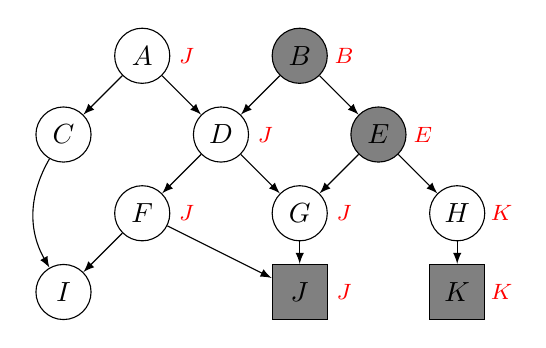
\begin{tikzpicture}[mynode/.style={circle,draw=black,fill=white,inner sep=0pt,minimum size=0.7cm},
      square/.style={rectangle,draw=black,fill=gray,inner sep=0pt,minimum size=0.7cm},
      graynode/.style={circle,draw=black,fill=gray,inner sep=0pt,minimum size=0.7cm},
      closurenode/.style={inner sep=0pt,minimum size=0.4cm,text=red,font=\footnotesize},
      >=latex]
      \node[mynode] (A) at (0,3) {$A$};
      \node[graynode] (B) at (2,3) {$B$};
      \node[mynode] (C) at (-1,2) {$C$};
      \node[mynode] (D) at (1,2) {$D$};
      \node[graynode] (E) at (3,2) {$E$};
      \node[mynode] (F) at (0,1) {$F$};
      \node[mynode] (G) at (2,1) {$G$};
      \node[mynode] (H) at (4,1) {$H$};
      \node[mynode] (I) at (-1,0) {$I$};
      \node[square] (J) at (2,0) {$J$};
      \node[square] (K) at (4,0) {$K$};
      \node[closurenode, anchor=west] at (A.east) {$J$};
      \node[closurenode, anchor=west] at (B.east) {$B$};
      \node[closurenode, anchor=west] at (C.east) {};
      \node[closurenode, anchor=west] at (D.east) {$J$};
      \node[closurenode, anchor=west] at (E.east) {$E$};
      \node[closurenode, anchor=west] at (F.east) {$J$};
      \node[closurenode, anchor=west] at (G.east) {$J$};
      \node[closurenode, anchor=west] at (H.east) {$K$};
      \node[closurenode, anchor=west] at (I.east) {};
      \node[closurenode, anchor=west] at (J.east) {$J$};
      \node[closurenode, anchor=west] at (K.east) {$K$};
      \draw[->] (A) -- (C);
      \draw[->] (A) -- (D);
      \draw[->] (B) -- (D);
      \draw[->] (B) -- (E);
      \draw[->] (D) -- (F);
      \draw[->] (D) -- (G);
      \draw[->] (E) -- (G);
      \draw[->] (E) -- (H);
      \draw[->] (F) -- (I);
      \draw[->] (F) -- (J);
      \draw[->] (G) -- (J);
      \draw[->] (H) -- (K);
      \draw[->,bend right=30] (C) to (I);
   \end{tikzpicture}
   } %
  \caption{Illustration of the connectors in a graph. The square nodes belong to $\mathbf{U}$, the connector of each node is written in red next to its node, and the LSCA closure $\Linfty(\mathbf{U})$ consists of the gray nodes.}
  \label{fig:c4example}
\end{figure}

Let us informally sketch the idea behind C4. By Lemma~\ref{lem:connectorunique}, it follows that the connector of $V$ is the unique node from $\Linfty (\mathbf{U})$ included in all paths from $V$ to $\Linfty (\mathbf{U})$. Assume $V \notin \mathbf{U}$. Then $V$ has access to $\mathbf{U}$ only via non-trivial paths, and the second node in each such path is a child of $V$.
Therefore, every path from $V$ to $\mathbf{U}$ must go through a node from the set $C$ of $V$'s children's connectors.
If $C=\emptyset$, $V$ has no path to $\mathbf{U}$, so $V \notin \Lambda(\mathbf{U},\mathbf{U})=\Linfty(\mathbf{U})$.
Furthermore, $V$ has no path to $\Linfty(\mathbf{U})$, so it has no connector.
If $C=\{X\}$, then all paths from $V$ to $\mathbf{U}$ must coincide at $X$, and again $V \notin \Lambda(\mathbf{U},\mathbf{U})=\Linfty(\mathbf{U})$.
Moreover, since $V \notin \Linfty(\mathbf{U})$, every path from $V$ to $\Linfty (\mathbf{U})$ must go through $X$, so $X$ is $V$'s connector.
If $|C|>1$, then one can show that there is a $\Lambda$-structure from $V$ to a pair of its children's connectors, and as these connectors are in $\Linfty(\mathbf{U})$, \Cref{prop:simple_graphical_charact} implies $V \in \Linfty (\Linfty(\mathbf{U}))$. However, it is easily seen that $\Linfty(\Linfty(\mathbf{U}))=\Linfty(\mathbf{U})$, so $V \in \Linfty(\mathbf{U})$ and is its own connector.
Accordingly, C4 sets $v \in \Linfty (U)$ iff $|C|>1$.
\Cref{prop:c4correct} formalizes our intuition, and \Cref{prop:c4runtime} establishes linear running time.

\begin{restatable}{theorem}{cfourcorrect}
   \label{prop:c4correct}
   C4 correctly computes $\Linfty(U)$.
\end{restatable}
\begin{restatable}{theorem}{cfourruntime}
   \label{prop:c4runtime}
   C4 runs in $O(|\mathbf{V}|+|E|)$ time.
\end{restatable}
In our experiments (\Cref{sec:experiments}), we accelerate C4 by preempting the computation of $C$ as soon as two members of $C$ are found, as this ensures $|C|>1$.
